\chapter{Sistemi noti}

\section{Equazione di Schrödinger per sistemi 1D}

\subsection{Particella libera}

Il sistema è descritto da

\begin{align}
H=\frac{p^2}{2m}
\end{align}

Ovviamente $[H,p]=0$, ed hanno quindi un insieme completo di autovettori simultanei. Essendo inoltre $p$ non degenere, ogni autovettore di $p$ corrisponderà ad un autovettore di $H$, con autovalori dati da

\begin{align}
p\ket{a}= p_a\ket{a} \quad \rightarrow \quad H\ket{a}= \frac{p_a^2}{2m}\ket{a}
\end{align}

Conseguentemente avremo anche

\begin{align}
|p'|= \sqrt{2mE}
\end{align}

Tuttavia notiamo una cosa: a questo valore del modulo corrispondono due autovettori, $\ket{p'}$ e $\ket{-p'}$!

Questo vuol dire che per data $E$ avremo

\begin{align}
H\ket{\psi}=E\ket{\psi}=E(\alpha\ket{p'} + \beta\ket{-p'})
\label{eq:key}
\end{align}

Possiamo trarre un po' di conseguenze da ciò:

\begin{enumerate}
	\item $H$ è degenere, e che quindi l'insieme dei $\ket{p'}$ è completo ma non costituisce la totalità degli autovettori, mentre l'insieme degli $\ket{\psi}$ sì.
	\item L'espressione \eqref{eq:key} presenta una nuova possibilità rispetto al caso classico: il corpo considerato può muoversi contemporaneamente in due direzioni!
	\item essendo i valori di $|p'|$ un insieme continuo avremo che anche lo spettro lo sarà. Ci troviamo quindi a lavorare con autovalori ed autovettori impropri, che dovremo quindi approssimare.
\end{enumerate}

Siccome ci troviamo a lavorare con l'impulso, poniamoci nella situazione di avere una misura il più precisa possibile. Scegliamo quindi di studiare il problema su una regione finita molto ampia, con una "superficie riflettente" posta a distanza L da degli estremi.
Avremo
\begin{align}
\Delta p \ll \frac{\hbar}{2 L } \ll 1
\end{align}

Possiamo quindi trascurare l'errore sull'impulso. 

Possiamo rappresentare la nostra particella in RS come 
$e^{+ikx}$, il che vuol dire che nel nostro "specchio" avremo $e^{-ikx}$.

I nostri treni d'onda sono molto lunghi, quindi per un periodo di tempo ci troviamo ad osservare entrambi i treni, e quindi, ci troveremo in una situazione del tipo

\begin{align}
{}&\psi= \alpha e^{+ikx} + \beta e^{-ikx} \\
&|\alpha|=|\beta|  
\end{align}

Quali saranno le autofunzioni?

\begin{align}
{}&H\psi= E\psi \rightarrow -\frac{\hbar^2}{2m} \frac{\partial^2}{\partial x^2}\psi = E\psi \\
&\downarrow \nonumber \\
&\psi''(x) + \frac{2mE}{\hbar^2}\psi(x)=0
\end{align}

Risolvendo l'equazione rappresentante avremo

\begin{align}
&\lambda^2 + \frac{2mE}{\hbar^2}\lambda=0 \nonumber \\
&\downarrow \nonumber \\
&\lambda = \pm i \sqrt{\frac{2mE}{\hbar^2}} \quad E \geq 0 \\
&\Lambda = \mp \sqrt{\frac{2mE}{\hbar^2}} \quad E < 0
\end{align}

Ricordando che le autofunzioni devono essere limitate dobbiamo per forza scartare il secondo caso, in quanto le soluzioni trovate con esso esplodono all'infinito.
\newpage

\subsection{Teorema di degenerazione e inversioni spaziali}

Il \textbf{teorema di degenerazione} afferma che:

\textit{date due osservabili $\eta$ e $\zeta$, se esse commutano con una terza osservabile $\xi$ ma non tra di loro, ovvero se
}

\smallskip

$[\xi, \eta]=[\xi, \zeta]= 0 \quad [\eta, \zeta]\neq 0$

\smallskip

\textit{allora $\xi$ è un'osservabile degenere.}

\bigskip

La dimostrazione giace nel fatto che se $\xi$ non fosse degenere allora \textbf{ogni suo autovettore dovrebbe esserlo anche di entrambe le altre osservabili}. Questo porterebbe ad avere un insieme di autovettori simultanei tra $\eta$ e $\zeta$, il che implicherebbe il loro commutare.

\bigskip

Applichiamo questo teorema al discorso della particella libera del paragrafo scorso. 

Sappiamo che gli autovalori di $H$ per $E>0$ sono doppiamente degeneri, e sappiamo che commuta con $p$. Possiamo quindi definire un terzo operatore che commuti con $H$ ma non con $p$. Introduciamo quindi l'\textbf{operatore di inversione spaziale}
$I$, definito in RS come

\begin{align}
I\psi_A(x)=\psi_A(-x)
\end{align}

dalle seguenti proprietà:

\begin{enumerate}
	\item $I^2= \mathbb{1}$ ovvero $I^2\psi_A(x)= \psi_A(x)$
	
	\item $I=I^\dagger$ ovvero $\braket{A|I|B}= \braket{B|I|A}^*$
	
		questo si vede dal fatto che
		
		\begin{align}
		\braket{A|I|B} {}&= \int dx \; \psi_A(x)^* I \psi_B(x) = \int dx \; \psi_A(x)^* \psi_B(-x) = \nonumber \\
		&= \left(\int dx \; \psi_B(-x)^* \psi_A(x) \right)^* = \nonumber \\
		&= \left(\int dx \; \psi_B(x)^* \psi_A(-x) \right)^* = \nonumber \\
		&= \left(\int dx \; \psi_B(x)^* I \psi_A(x)\right)^* = \braket{B|I|A}^*
		\end{align}
		
	\item Da queste due segue anche che è unitario, ovvero $I^\dagger = I^{-1}$
	
	\item $I\psi_I(x)= \pm \psi_I(x)$ dato che
	
		\begin{align}
		{}&I\psi_I(x) = w \psi_I(x) \nonumber \\
		&\downarrow \nonumber \\
		&I^2\psi_I(x) = w I\psi_I(x) \nonumber \\
		&\downarrow \nonumber \\
		&\psi_I(x) = w^2\psi_I(x) \rightarrow w^2=1 \rightarrow w= \pm 1
		\end{align}
	
	\item Le autofunzioni di I $\psi_I(x)$ saranno dunque divise in due famiglie:
	
		\begin{enumerate}
		\item \textbf{Pari} ($w=+1$) ovvero tali che $\psi_I(x)=+\psi_I(-x)$
		\item \textbf{Dispari} ($w=-1$) ovvero tali che $\psi_I(x)=-\psi_I(-x)$
		\end{enumerate}
	
	\item Le $\psi_I(x)$ costituiscono un insieme completo. Ogni $\psi(x)$ può espressa come combinazioni di $\psi_I(x)$ pari e dispari grazie all'identità
	
	\begin{align}
	\psi(x)= \frac{1}{2}(\psi(x) + \psi(-x)) + \frac{1}{2}(\psi(x) - \psi(-x))
	\end{align}
	Dove la prima delle due è pari e la seconda dispari
	
	\item  $I$ anticommuta con $q$ e $p$:
	
	\begin{align}
	{}&IqI^{-1}= -q \quad ; \quad IpI^{-1} = -p \\
	&Iq= -qI \quad ; \quad Ip= -pI
	\end{align}
	
	Dimostriamolo per $q$:
	\begin{align}
	Iq\ket{A} \rightarrow I(x\psi_A(x))= -x \psi_A(-x)= -xI\psi_A(x) \rightarrow-qI\ket{A}  
	\end{align}	

	Analogamente per $p$:
	\begin{align}
	{}& Ip\ket{A} \rightarrow I \left(-i\hbar \frac{\partial}{\partial x}\psi_A(x)	\right)= -i\hbar \frac{\partial}{\partial x}\psi_A(-x) 	\\
	& pI \ket{A}  \rightarrow -i\hbar \frac{\partial}{\partial x}\psi_A(-x)= i\hbar \frac{\partial}{\partial x}\psi_A(x) 
	\end{align}
	Da cui segue il risultato.

\end{enumerate}

Queste proprietà si trasferiscono inalterate al caso in più dimensioni $I\psi(q_1, ..., q_n)= \psi(-q_1,...,-q_n)$.

Questo operatore così definito commuta con l'energia cinetica 

\begin{align}
I\frac{p^2}{2m}I^{-1} = \frac{1}{2m} IpI^{-1}IpI^{-1}= \frac{1}{2m} (-p)^2= \frac{p^2}{2m}
\end{align}


e con tutte le osservabili del tipo $f(q,p) : f(q,p)=f(-q,-p)$ dato che

\begin{align}
If(q,p)I^{-1}=f(-q,-p)
\end{align}

E quindi con tutte le Hamiltoniane della famiglia $V(q)= V(-q)$.

\bigskip

Siccome $I$ e $p$ commutano entrambi con $H$ ma non tra di loro ne segue che quest'ultima deve essere un'osservabile degenere.


Sia ora $\ket{p'}$ un autovettore simultaneo di $H$ (corrispondente all'autovalore $E$) e $p$ tale che

\begin{align}
I\ket{p'} = \ket{-p'}
\end{align}

Sappiamo che $\ket{-p'}$ è ancora autovettore di $E$, essendo sullo stesso raggio di vettori di $\ket{p'}$.

Ma sappiamo anche che se $p'\neq 0$ allora $\braket{-p'|p'}=0$ e quindi $E$ è degenere almeno due volte. 

Applicando di nuovo $I$ a $\ket{-p'}$ non si ottiene un nuovo vettore, e quindi la degenerazione di ferma a 2.

IL discorso si può fare anche partendo da $H$ ed $I$ e applicando $p$, e si ricava ugualmente la doppia degenerazione.

\newpage

\subsection{L'equazione di Schrödinger}

L'espressione generale avrà forma

\begin{align}
H= \frac{1}{2m} p^2 + V(x)
\end{align}

Le cui soluzioni possono essere trovate nel seguente modo:

\begin{align}
{}&-\frac{\hbar^2}{2m} \frac{\partial^2}{\partial x^2}\psi(x) + V(x)\psi(x) = E\psi(x) \\
&\downarrow \nonumber \\
& \psi''(x) -\frac{2m}{\hbar^2} (V(x)-E)\psi(x)=0
\end{align}

Ci troviamo quindi con due casi:

\begin{enumerate}
	\item $\psi(x)\in L^2$, limitate e a supporto compatto (autofunzioni proprie)
	\item $\psi(x)\notin L^2$, $\psi(x) \,$ limitate (autofunzioni improprie a spettro continuo)
\end{enumerate}

notiamo come essendo l'equazione a coefficienti reali avremo che se $\psi(x)$ è soluzione allora anche $\psi^*(x)$ lo è.

Fissato ora il valore di $E$ avremo due casi:

\begin{enumerate}
	\item $V(x)-E<0$
	
	In questo caso si ha che 
	
	\begin{align}
	V(x)<E \rightarrow  \frac{\psi''}{\psi}<0 \rightarrow 
	\left\{
	\begin{array}{cc}
	\psi''(x) >0 \, , \, \psi(x)<0 \\
	\psi''(x) <0 \, , \, \psi(x)>0
	\end{array}
	\right.
	\end{align}
	
	Ci troviamo a lavorare con le cosidette \textbf{regioni di tipo I}:
	
	\begin{figure}[!htb]
		\center{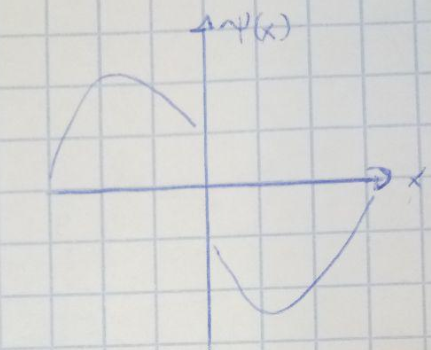
\includegraphics[width=.5\textwidth]
			{images/TipoI.png}
			\caption{esempio di regione}}
	\end{figure}
	\newpage
	
	\item $V(x)-E>0$
	
	\begin{align}
	V(x)>E \rightarrow  \frac{\psi''}{\psi}<0 \rightarrow 
	\left\{
	\begin{array}{cc}
	\psi''(x) >0 \, , \, \psi(x)>0 \\
	\psi''(x) <0 \, , \, \psi(x)<0
	\end{array}
	\right.
	\end{align}
	
	E si parla di  \textbf{regioni di tipo II}:
	
	\begin{figure}[!htb]
		\center{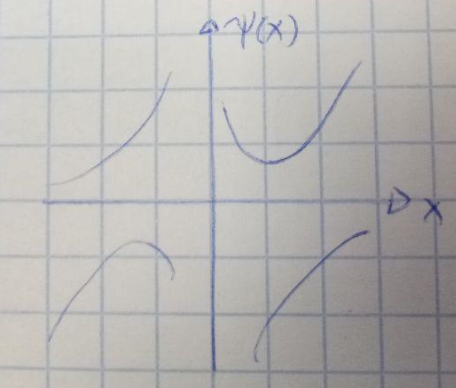
\includegraphics[width=.5\textwidth]
			{images/TipoII.png}
			\caption{esempio di regione}}
	\end{figure}
	
	
	\item $V(x)=E$ 

	  Si parla qui di \textbf{punti di inversione} da tipo I a tipo II e viceversa.
\end{enumerate}

\newpage

\subsection{Soluzioni dell'equazione di Schrödinger}

\subsubsection{Autovalori discreti}

Studiamo un sistema dove $\lim_{x \rightarrow \pm \infty}V(x)= +\infty$

Ci torveremo con due casi:

\begin{enumerate}
	\item $E<V_{\text{min}}$
	
	In questo caso $E<V(x) \; \forall x$, e si avranno quindi solo regioni di tipo II, con conseguente assenza di spettro discreto.
	
	\item $E>V_{\text{min}}$

	In questo caso ci troviamo ad avere entrambe le regioni

		\begin{align}
			\left\{
			\begin{array}{cc}
				E> V(x) \quad x \in [x_1 , x_2] \quad \text{tipo I }\\
				E< V(x) \quad x \notin [x_1 , x_2] \quad \text{tipo II}
			\end{array}
			\right.
		\end{align}

	e le nostre soluzioni si troveranno nelle regioni di tipo I.
\end{enumerate}

Le nostre soluzioni saranno tali che

\begin{align}
{}&\lim_{x \rightarrow \pm \infty} \psi(x)=0 \quad x \notin [x_1, x_2] \\
& \text{oppure} \nonumber \\
&\lim_{x \rightarrow \pm \infty} \psi(x)=\pm \infty \quad x \notin [x_1, x_2]
\end{align}

Ovvero nelle regioni di tipo II non può oscillare o rimanere limitata senza convergere a 0.

Cerchiamo di capire come ottenere soluzioni accettabili. 

Supponiamo di avere 

\begin{align}
\psi(x_0)>0 \quad ; \quad x_o<x_1
\end{align}

In questo caso ci basta fissare $\psi'(x_0)$ per risolvere il problema.

Ci troveremo con 3 casi:

\begin{enumerate}
	\item $\psi'(x_0)>0$ ma piccolo oppure $\psi'(x_0)<0$
	
	In questo caso avremo 
	\begin{align}
	\lim_{x \rightarrow -\infty}\psi(x)=+\infty \quad ; \quad \psi(x)\neq 0 \;\; \forall x
	\end{align}
	
	
	\item $\psi'(x_0)>0$ grande

	In questo caso avremo 
	\begin{align}
	\lim_{x \rightarrow -\infty}\psi(x)=-\infty \quad ; \quad \psi(x_a)= 0 \;\; x=x_a
	\end{align}
	
	\item $\psi'(x_0)>0$ nella media tra 1 e 2
	
	In questo caso avremo 
	\begin{align}
	\lim_{x \rightarrow -\infty}\psi(x)=0 \quad ; \quad \psi(x) \neq 0 \;\; \forall x
	\end{align}
		
\end{enumerate}

Ovviamente il tipo di soluzioni che fanno comodo a noi sono quelle del tipo 3.

Supponiamo ora per semplicità che tutto l'intervallo $[x_1,x_2]$ sia una sola regione di tipo I, e vediamo come si comporta per $x\rightarrow +\infty$.

Dentro $[x_1,x_2]$ avremo un comportamento oscillante di $\psi(x)$.

\newpage

Qualora ci troviamo in una situazione tale per cui $E>V(x)$ ma di poco, La $\psi(x)$ non si annulla mai, e avremo tre casi:

\begin{enumerate}
	\item $\lim_{x \rightarrow +\infty}\psi(x)=+\infty$
	
	\begin{figure}[!htb]
		\center{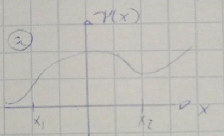
\includegraphics[width=0.3\textwidth]
			{images/I.png}
			\caption{\label{fig:my-label}}}
	\end{figure}
	In questo caso E non sarà autovalore valido, non essendo $\psi(x)$ a supporto compatto, e avremo $E_1<E_2$

	\item $\lim_{x \rightarrow +\infty}\psi(x)=0$

	\begin{figure}[!htb]
		\center{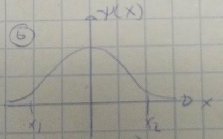
\includegraphics[width=0.3\textwidth]
			{images/II.png}
			\caption{\label{fig:my-label}}}
	\end{figure}
	In questo caso invece abbiamo invece una soluzione valida, a cui corrisponderà un valore ben distinto.
	
	\item $\lim_{x \rightarrow +\infty}\psi(x)=-\infty$

	\begin{figure}[!htb]
		\center{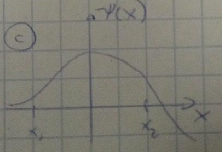
\includegraphics[width=0.3\textwidth]
			{images/III.png}
			\caption{\label{fig:my-label}}}
	\end{figure}

	Anche qui non abbiamo una soluzione valida per lo stesso motivo di 1, con $E_3>E_2$.
\end{enumerate}


Ricordando che 

\begin{align}
\psi''(x) = \frac{2m}{\hbar^2}(V(x)-E)\psi(x)
\end{align}


Notiamo come partendo da $E=V_{min}$ e incrementando valori di $E$ si passerà con continuità dal caso 1 al caso 3, e nel mezzo ci sarà sempre un insieme discreto che restituisce soluzioni accettabili.

Un'altra conseguenza è che l'autofunzione corrispondete al valore più basso di E non si annulla mai al finito, e quindi \textbf{non ha nodi}.

Aumentando l'energia si spostano i punti di inversione $x_1$ e $x_2$ rispettivamente a sinistra e a destra, e aumenta la curvatura di $\psi(x)$ all'interno, e conseguentemente il numero di volte che la funzione oscilla (ovvero attraversa l'asse x).

\newpage

Il fatto che le autofunzioni degli stati eccitati debbano avere nodi viene da fatto che 

\begin{align}
\int \psi_0(x)\psi_n(x)=0
\end{align}

e visto che $\psi_0(x)>0 \, \forall x$ per forza di cose devono potersi annullare, e quindi avere nodi le altre. QUesto ci porta ad enunciare il

\bigskip

\textbf{Teorema dei nodi:} 

\textit{Per un sistema con un solo grado di libertà e spettro discreto:}

\smallskip

$H\psi_0(x)= E_0\psi_0(x)$

$H\psi_1(x)= E_0\psi_1(x)$

...

$H\psi_n(x)= E_n\psi_n(x)$
\smallskip

\textit{Il numero di nodi di $\psi_n(x)$ viene dato dal numero quantico principale $n$.}

\bigskip

L'ultimo problema da risolvere per gli autovalori discreti è quello della degenerazione, che viene affrontato con il 


\textbf{Teorema della non degenerazione:}

\textit{Per ogni sistema 1D gli autovalori discreti della Hamiltoniana sono non degeneri.}

\bigskip

Questo si dimostra rapidamente prendendo in cosiderazione due autofunzioni qualsiasi $\psi_1(x)$ e $\psi_2(x)$ corrispondenti allo stesso autovalore $E$:

\begin{align}
\psi_1''(x) = \frac{2m}{\hbar^2}(V(x)-E)\psi_1(x) \\
\psi_2''(x) = \frac{2m}{\hbar^2}(V(x)-E)\psi_2(x)
\end{align}

Moltiplicando l'una per la $\psi(x)$ dell'altra e sottraendo membro a membro otteniamo che 

\begin{align}
\psi_1''(x)\psi_2(x) - \psi_1(x)\psi''_2(x)=0
\end{align}

che è uguale a scrivere

\begin{align}
\frac{\partial}{\partial x}(\psi_1'(x)\psi_2(x) - \psi_1(x)\psi'_2(x))=0
\end{align}

che, integrando porta a scrivere

\begin{align}
\psi_1'(x)\psi_2(x) - \psi_1(x)\psi'_2(x)= cost.
\end{align}

Ma $E$ è un autovalore discreto, e quindi le autofunzioni si annullano per $x \rightarrow \pm \infty$, e quindi $cost.=0$

questo ci porta a

\begin{align}
{}&\psi_1'(x)\psi_2(x) = \psi_1(x)\psi'_2(x) \\
&\downarrow \nonumber \\
&\frac{\psi_1'(x)}{\psi_1(x)}=\frac{\psi_2'(x)}{\psi_2(x)}\\
&\downarrow \nonumber \\
& \frac{\partial}{\partial x} \ln{\psi_1(x)} =  \frac{\partial}{\partial x}\ln{\psi_2(x)}
\end{align}

Integrando otteniamo che

\begin{align}
\psi_1(x) = C \psi_2(x)
\end{align}
e che quindi le due autofunzioni non sono indipendenti ed $E$ non è degenere.

Consideriamo ora un caso molto importante: $V(x)=V(-x)$

In questo caso avremo che $[H,I]=0$, e quindi ci sarà un insieme di autofunzioni simultanee.

Gli autovalori discreti $E$ sono non degeneri, e siccome ogni autofunzione di H corrispondente ad E è anche tale di $I$ deve avere anche parità definita.

Notiamo ora che

\begin{enumerate}
	\item Le funzioni \textbf{pari} hanno o un numero pari di nodi o infinito, in quanto se si annulla per dato $x_0$ si deve annullare anche a $-x_0$
	\item Le funzioni \textbf{dispari} hanno o un numero dispari di nodi o infinito, dovendosi annullare anche nell'origine per definizione, mentre se le pari se si annullano nell'origine hanno uno zero di ordine pari
\end{enumerate}

Però le soluzioni dell'eq di Schrödinger non possono avere zeri di ordine superiore al primo: se in un punto si annullano sia $\psi(x)$ che $\psi'(x)$ allora la soluzione è ben definita ed è quella identicamente nulla.

Ricordando anche il teorema dei nodi possiamo concludere dicendo che \textbf{la parità delle autofunzioni è data dal numero quantico principale $n$, con quella dello stato fondamentale sempre pari}.

\newpage

\subsubsection{Autovalori continui}

Consideriamo ora il seguente potenziale:

\begin{align}
\lim V(x)=
\left\{
\begin{array}{cc}
+\infty \quad x\rightarrow-\infty \\
0 \;\,\qquad x\rightarrow +\infty
\end{array}
\right.
\end{align}

	\begin{figure}[!htb]
	\center{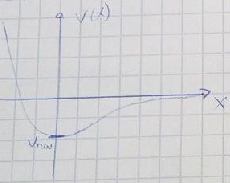
\includegraphics[width=0.3\textwidth]
		{images/contI.png}
		\caption{\label{fig:my-label}}}
\end{figure}

Ci troveremo a lavorare con tre casi:

	\begin{figure}[!htb]
	\center{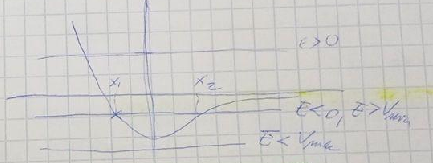
\includegraphics[width=0.3\textwidth]
		{images/contII.png}
		\caption{\label{fig:my-label}}}
\end{figure}

\begin{enumerate}
	\item $E<V_{min}$ 
	
	In questo caso tutto l'asse x  è una regione di tipo II e non sono ammessi autovalori.
	
	\item $V_{min}<E<0$ 
	
	In questo caso avremo solo autovalori discreti in una regione compresa tra due punti. Notiamo che per la forma del potenziale avremo la soluzione generale sarà della forma
	
	\begin{align}
	\alpha e^{\sqrt{sm|E|} \frac{x}{\hbar}} + \beta e^{-\sqrt{sm|E|} \frac{x}{\hbar}} \\
	\alpha, \beta \in \mathbb{C} \quad; \quad x\rightarrow +\infty
	\end{align}
	
	In questo caso, per $E$ fissato e scelta una soluzione che si annulla per $x\rightarrow -\infty$, di norma si ha una soluzione con entrambi i coefficienti $\neq 0$, ma è solo per quelle con $\alpha =0$ che si hanno soulzioni accettabili ed $E$ è autovalore di $H$.
	
	Il numero di autovalori dipende da $V(x)$. 
	
	In particolare \textbf{se $\lim_{x\rightarrow +\infty}V(x)\ll \lim_{x\rightarrow +\infty}x^{-2}$ e $V(x)$ limitata inferiormente allora  il numero di autovalori dell'energia sarà finito od eventualmente nullo}.
	
	\item $E>0$
	
	In questo caso per $x\ll 0$ avremo una regione di tipo II e per $x \gg 0$ saranno di tipo I. Sarà quindi possibile trovare una soluzione del tipo
	
	\begin{align}
	\alpha e^{i\sqrt{2mE} \frac{x}{\hbar}} + \beta e^{-i\sqrt{smE} \frac{x}{\hbar}} \\
	\alpha, \beta \in \mathbb{C} \quad; \quad x\rightarrow +\infty
	\end{align}
	
	E quindi sempre accetabile. Notiamo come al contrario dei casi precedentemente studiati non serve che la $\psi(x)$ si annulli per $x\rightarrow +\infty $, in quanto rimane comunque limitata. Abbiamo quindi che ogni $E>0$ è autovalore improprio di $H$ e ci troviamo in presenza di uno \textbf{spettro continuo}, in questo caso non degenere.
	\end{enumerate}

Un ultimo caso da considerare è il seguente:

\begin{align}
\lim V(x)=
\left\{
\begin{array}{cc}
V_1 \quad x\rightarrow -\infty \\
V_2 \quad x\rightarrow +\infty
\end{array}
\right. \quad ; \quad V_min<V_1<V_2
\end{align}

\begin{figure}[!htb]
	\center{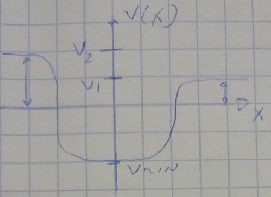
\includegraphics[width=0.5\textwidth]
		{images/contIII.png}
		\caption{\label{fig:my-label}}}
\end{figure}

Avremo qui 4 casi:

\begin{enumerate}
	\item $E<V_{min}$
	
	In questo caso non si hanno autovalori validi
	
	\item $V_{min}<E<V_1$
	
	Per $|x|\gg 0$ ho regioni di tipo II con in mezzo almeno una regione di tipo I, e quindi abbiamo solo autovalori discreti
	
	\item $V_1<E<V_2$
	
	Per $x \ll 0$ abbiamo una regione di tipo II, mentre per $x \gg 0$ ne avremo una di tipo I con tutti valori $E>0$, continui e non degeneri. È il caso speculare del caso 2 del precedente potenziale, e stavolta nella soluzione porremo $\beta=0$
	
	\item $E>V_2$
	
	Per $|x|\gg 0$ avremo regioni di tipo I, in mezzo dipende dalla forma di $V(x)$.
		Avremo 
	
	\begin{align}
	\psi(x)= \left\{
	\begin{array}{cc}
	\alpha e^{+i\frac{\sqrt{2m(E-V_2)}}{\hbar}}x + \beta e^{-i \frac{\sqrt{2m(E-V_2)}}{\hbar}x} \quad;\quad  x\rightarrow -\infty \\
	\gamma e^{+i \frac{\sqrt{2m(E-V_1)}}{\hbar}x} + \delta e^{-i \frac{\sqrt{2m(E-V_1)}}{\hbar}x} \quad;\quad  x\rightarrow +\infty \\
	\end{array}
	\right.
	\end{align}
	E tutte le soluzioni sono valide e per $E>V_2$ avremo uno spettro continuo 2 volte degenere, non essendo i coefficienti indipendenti.
\end{enumerate}

In generale si può dire che

\begin{enumerate}
	\item Tutto l'asse x di tipo II: no autovalori
	\item $x\rightarrow \pm \infty$ di tipo II: spettro discreto non degenere
	\item $x\rightarrow \pm \infty$ di tipo I $x\rightarrow \mp \infty$ di tipo II: spettro continuo non degenere
	\item $x\rightarrow \pm \infty$ di tipo I: spettro continuo 2 volte degenere
\end{enumerate}


\newpage
\section{L'oscillatore armonico (Caso 1D)}

L'oscillatore armonico viene descritto dall'Hamiltoniana:

\begin{align}
H = \frac{1}{2m} p^2  + \frac{1}{2} m \omega^2 q^2
\end{align}

Per la quale valgono le seguenti proprietà:

\begin{enumerate}
	\item i suoi autovalori sono tutti positivi, infatti, preso un $\ket{A}$ nomralizzato
	
	\begin{align}
	E=\overline{H}= \braket{A |H| A} \propto \braket{A |p^2| A}  + \braket{A |q^2| A} = |p \ket{A}|^2 +  |q\ket{A}|^2
	\end{align}
	
	essendo entrambi moduli sono entrambi $\geq 0$ per definizione, da cui segue che anche $\overline{H}$ lo è. Ma c'è un problema!
	
	\begin{align}
	E={}&\overline{H}=0 \rightarrow \braket{A |p^2| A}  + \braket{A |q^2| A} = 0 \nonumber \\
	&\downarrow\nonumber \\
	&\braket{A |p^2| A}  = -\braket{A |q^2| A} \nonumber \\
	&\downarrow\nonumber \\
	&\braket{A |p^2| A}  = \braket{A |q^2| A} = 0
	\end{align}
	
	Questo è impossibile, visto che $[q,p]=i\hbar$, questo implica che 
	
	\begin{align}
	E > 0
	\end{align}
	
	\item $\braket{A |q| A} = 0 = \braket{A |p| A}$
	
	 questo viene dimostrato dal fatto che
	 
	 \begin{align}
	 [V(q), q]=0 \rightarrow  [H,q]= \frac{1}{2m}[p^2,q]
	 \end{align}
	 ricordando le proprietà dei commutatori e la relazione di indeterminazione otteniamo
	 
	 \begin{align}
	 [p^2,q] = p[p,q] + [p,q]p= 2i\hbar p
	 \end{align}
	 
	 e quindi
	 \begin{align}
	 [H,q]= -\frac{i \hbar}{m}p
	 \end{align}
	 
	 calcolandone il valore medio su un autostato di H otteniamo
	 
	 \begin{align}
	 \braket{E_n|[H,q]|E_n} = \left\{
	 \begin{array}{cc}
		-\frac{i \hbar}{m}p \\
		\braket{E_n|Hq - qH|E_n}
	 \end{array}
	 \right.
	 \end{align}
	 
	 ma abbiamo anche che, ricordando che H è hermitiana,
	 \begin{align}
	{}&\braket{E_n|Hq - qH|E_n} = \braket{E_n|Hq|E_n} - \braket{E_n|qH|E_n} \\ 
	&\downarrow \nonumber \\
	&E_n\braket{E_n|q|E_n} - \braket{E_n|q|E_n}E_n=0
	 \end{align}

	da cui $\braket{E_n|p|E_n}=0$. Si dimostra allo stesso modo calcolando $[H,p]$ che anche $\braket{E_n|q|E_n}=0$.

\item $E_0 \geq \frac{1}{2} \hbar \omega$
	\begin{align}
	{}&\braket{E_0|E_0}=1 \\
	 &\downarrow \nonumber \\ 
	 &E_0= \braket{E_0|H|E_0}= \frac{1}{2m}\braket{E_0|p^2|E_0} + \frac{m\omega^2}{2}\braket{E_0|q^2|E_0} \\
	 &\downarrow \nonumber \\ 
	 &E_0=  \frac{1}{2m}(\Delta p)^2 + \frac{m\omega^2}{2}(\Delta q)^2 \geq \omega \Delta p \Delta q = \frac{1}{2}\hbar \omega
	 \end{align}
	 
	 l'ultimo passaggio è dovuto alla disuguaglianza triangolare e al principio d'indeterminazione.
\end{enumerate}

\subsection{Spettro e autovettori dell'oscillatore armonico}

Per descrivere lo spettro introduciamo gli operatori non hermitiani detti di \textbf{discesa} e \textbf{salita}:

\begin{align}
\eta = \frac{1}{\sqrt{2m\omega\hbar}}(p - im\omega q) \quad ; \quad \eta^\dagger =\frac{1}{\sqrt{2m\omega\hbar}}(p + im\omega q)
\end{align}

da cui ricaviamo

\begin{align}
q= -\i \sqrt{\frac{\hbar}{2m\omega}}(\eta^\dagger - \eta )  \quad ; \quad p = \sqrt{\frac{m\hbar\omega}{2}}(\eta^\dagger + \eta ) 
\end{align}

o, come si trova in altri testi come il Patrì-Testa (noi useremo la prima definizione, ma per completezza riportiamo anche questa):

\begin{align}
a= \sqrt{\frac{m\omega}{2\hbar}}(q+ \frac{i}{m\omega}p)\quad &; \quad a^\dagger = \sqrt{\frac{m\omega}{2\hbar}}(q- \frac{i}{m\omega}p) \\
q= \sqrt{\frac{\hbar}{2m\omega}}(a + a^\dagger) \quad &; \quad p= i\sqrt{\frac{m\omega \hbar}{2}}(a - a^\dagger)
\end{align}

Iniziamo calcolando quantità utili per le prossime dimostrazioni:

\begin{align}
\eta^\dagger \eta {}&= \frac{1}{2m\omega\hbar}[p^2 + (m\omega)^2 q^2 + im\omega(qp - pq)]= \nonumber \\
& = \frac{1}{2m\omega\hbar}(p^2 + (m\omega)^2 q^2 + im\omega[q,p])= \nonumber \\
&= \frac{1}{2m\omega\hbar}(p^2 + (m\omega)^2 q^2 + im\omega i\hbar)= \nonumber \\
&= \frac{1}{2m\omega\hbar}(p^2 + (m\omega)^2 q^2 - m\omega\hbar) = \nonumber \\
&= \frac{1}{\hbar\omega}\left(\frac{1}{2m}p^2 + \frac{m\omega^2}{2} q^2\right) - \frac{1}{2}= \frac{1}{\hbar\omega}H -\frac{1}{2} \\
\nonumber \\
\eta \eta^\dagger &= \frac{1}{\hbar\omega}H +\frac{1}{2}
\end{align}

\newpage 
Da cui otteniamo: 

\begin{align}
{}&H =\hbar\omega \, \eta^\dagger \eta + \frac{\hbar\omega}{2} \\
&[\eta,\eta^\dagger]=1 \\
&[H,\eta]= \hbar\omega [\eta^\dagger \eta, \eta]= -\hbar\omega \eta \\
&[H,\eta^\dagger]= \hbar\omega [\eta^\dagger \eta, \eta^\dagger]= \hbar\omega \eta
\end{align}

Vediamo ora perché il nome degli operatori introdotti. Iniziamo con quello di \textbf{discesa}:

\begin{align}
H\eta\ket{E_n} {}&= ([H,\eta] +\eta H)\ket{E_n}= (-\hbar\omega \eta + +\eta H)\ket{E_n}= \nonumber \\
&= -\hbar\omega \eta \ket{E_n} + \eta H \ket{E_n} = -\hbar\omega \eta \ket{E_n} + \eta E_n \ket{E_n}=\nonumber \\
&=  (E_n-\hbar \omega) \eta \ket{E_n}
\end{align}

Notiamo come $\eta \ket{E}$ sia ancora autovalore di H, ma di un livello ad energia più bassa!

considerando il terzo punto dello scorso paragrafo, dovremo avere un'energia minima, che troviamo nel seguente modo: 

\begin{align}
{}&E \geq 0 \rightarrow \exists E_0: \eta \ket{E_0}=0 \\
&\downarrow \nonumber \\
&0=\bra{E_0}\eta^\dagger\eta \ket{E_0} = \braket{E_0|\frac{1}{\hbar\omega}H -\frac{1}{2}|E_0}= \frac{1}{\hbar\omega}E_0 -\frac{1}{2} \nonumber\\
&\downarrow \nonumber \\
& E_0= \frac{1}{2}\hbar\omega
\end{align}

Mentre invece non c'è un valore massimo possibile, infatti

\begin{align}
{}&0=\bra{E_{max}}\eta\eta^\dagger \ket{E_{max}} = \braket{E_{max}|\frac{1}{\hbar\omega}H +\frac{1}{2}|E_{max}}= \frac{1}{\hbar\omega}E_{max}+\frac{1}{2} \nonumber\\
&\downarrow \nonumber \\
& E_{max}= -\frac{1}{2}\hbar\omega
\end{align}

che è impossibile. 
 
Possiamo quindi ricavare lo spettro, applicando n volte $\eta^\dagger$ a $E_0$, ottenendo

\begin{align}
E_n= \left(\frac{1}{2}+n\right)\hbar\omega
\end{align}

Notiamo anche che che

\begin{align}
E_n-\hbar \omega = \left(\frac{1}{2}+n - 1\right)\hbar\omega \\
E_n+\hbar \omega = \left(\frac{1}{2}+n + 1\right)\hbar\omega
\end{align}

\newpage
Da cui segue che, chiamati gli autovettori $\ket{n}$

\begin{align}
\eta \ket{n}=\sqrt{n}\ket{n- 1}\\
\eta^\dagger  \ket{n}= \sqrt{n+1}\ket{n+ 1}
\end{align}

Definiamo così gli autostati normalizzati

\begin{align}
\ket{n}= \frac{(\eta^\dagger)^n}{\sqrt{n!}}\ket{0}
\end{align}


\subsection{L'oscillatore armonico 1D in RS}

Come possiamo esprimere l'oscillatore armonico in uno spazio $L_2$?

Una via è la risoluzione dell'equazione di Schrödinger:

\begin{align}
-\frac{\hbar^2}{2m}\psi_n''(x)+\frac{m\omega^2x^2}{2}\psi_n(x)=E_n\psi_n(x) 
\end{align}

Ma c'è una via più semplice! Infatti abbiamo che

\begin{align}
{}&\ket{n}= \frac{(\eta^\dagger)^n}{\sqrt{n!}}\ket{0} \rightarrow \psi_n(x)= \braket{x|n}= \frac{(-1)^n}{\sqrt{n!}}\braket{x|\eta^\dagger|0} \\
\nonumber \\
&\eta^\dagger = \frac{1}{\sqrt{2m\omega\hbar}}(p + im\omega q) \rightarrow \eta^\dagger= \frac{1}{\sqrt{2m\omega\hbar}} \left( -i\hbar \frac{\partial}{\partial x} + im\omega x \right)
\end{align}

Da cui ricaviamo

\begin{align}
\psi_n(x)= \frac{(2m\omega \hbar)^{\frac{n}{2}}}{\sqrt{n!}}\left( -\hbar \frac{\partial}{\partial x} + m\omega x \right)^n \psi_0(x)
\end{align}


ma come troviamo $\psi_0(x)$?

Ricordando che $\ket{0}: \eta\ket{0}=0$ avremo

\begin{align}
\left( \hbar \frac{\partial}{\partial x} + m\omega x \right) \psi_0(x) =0
\end{align}

Che è un'eqauzione differenziale al primo ordine che possiamo risolvere senza problemi!

\begin{align}
{}&\hbar \psi'_0(x) + m\omega x \psi_0(x)=0 \nonumber \\
& \downarrow \nonumber \\
& \frac{\partial \psi_0(x)}{\psi_0(x)} = -\frac{m\omega}{\hbar} x \partial x  \nonumber \\
& \downarrow \nonumber \\
& \int_{\psi_0(0)}^{\psi_0(x)} \frac{\partial \psi_0(x)}{\psi_0(x)} = -\frac{m\omega}{\hbar} \int_{0}^{x} \partial x \; x  \nonumber \\
& \downarrow \nonumber \\
& \ln(\frac{\psi_0(x)}{\psi_0(0)}) = -\frac{m\omega}{2\hbar}x^2 \nonumber \\
& \downarrow \nonumber \\
& \psi_0(x) = \psi_0(0) e^{-\frac{m\omega}{2\hbar}x^2}
\end{align}

(nota: chiamare gli estremi di integrazione e la variabile di integrazione con lo stesso nome è un vizio di forma per non confondere il lettore introducendo troppe variabili).

Per trovare $\psi_0(0)$ ci basta normalizzare:

\begin{align}
{}&|\psi_0(x)|^2 = 1 = \int_{-\infty}^{+\infty} |\psi_0(0)|^2 e^{-\frac{m\omega}{\hbar}x^2} \nonumber \\
& \downarrow \nonumber \\
&1=|\psi_0(0)|^2 \int_{-\infty}^{+\infty}  e^{-\frac{m\omega}{\hbar}x^2} = |\psi_0(0)|^2 \sqrt{\frac{\hbar \pi}{m \omega}}\nonumber \\
& \downarrow \nonumber \\
&|\psi_0(0)|^2 \sqrt{\frac{\hbar \pi}{m \omega}}=1 \rightarrow \psi_0(0)= \sqrt[4]{\frac{\hbar \pi}{m \omega}}
\end{align}

E possiamo quindi scrivere

\begin{align}
\psi_0(x) = \sqrt[4]{\frac{\hbar \pi}{m \omega}} e^{-\frac{m\omega}{2\hbar}x^2}
\end{align}

In conclusione scriviamo quindi

\begin{align}
\psi_n(x)= \frac{(2m\omega \hbar)^{-\frac{n}{2}}}{\sqrt{n!}}\left( -\hbar \frac{\partial}{\partial x} + m\omega x \right)^n \sqrt[4]{\frac{\hbar \pi}{m \omega}} e^{-\frac{m\omega}{2\hbar}x^2}
\end{align}

Possiamo anche scrivere il tutto in modo più compatto introducendo i \textbf{polinomi di Hermite}:

\begin{align}
H_n(\xi) = e^{\frac{\xi^2}{2}} \left( -\frac{\partial}{\partial \xi} + \xi \right)^n e^{-\frac{\xi^2}{2}}
\end{align}

e ponendo $\xi = \sqrt{-\frac{m\omega}{2\hbar}}x$, ottenendo in conclusione:

\begin{align}
\psi_n(x)= \frac{1}{\sqrt{2^n n!}}\sqrt[4]{\frac{\hbar \pi}{m \omega}}H_n\left(\sqrt{-\frac{m\omega}{2\hbar}}x\right) e^{-\frac{m\omega}{2\hbar}x^2}
\end{align}

\newpage

\section{L'oscillatore armonico (Caso 3D)}

Nel caso 3D H assume la forma

\begin{align}
H= \frac{1}{2m}p^2 + \frac{m\omega^2}{2}q^2 \quad;\quad 
\left\{
\begin{array}{cc}
p^2= p_x^2 + p_y^2 + p_z^2 \\
q^2= x^2 + y^2 + z^2
\end{array}\right.
\end{align}

In questo caso V(q) fa parte della famiglia dei \textbf{potenziali centrali}, che studiamo nel prossimo capitolo, e quindi come vederemo gli autovettori ed autofunzuoni potranno essere espresse come
\begin{align}
\ket{E,l,m} \leftrightarrow \psi_{elm}(q)
\end{align}

Invece di risolvere l'equazione di Schrödinger, che richiederebbe numerosi conti, possiamo riscrivere H \textbf{separando le variabili}!

\begin{align}
H{}&=\left(\frac{1}{2m} p_x^2  + \frac{m \omega^2}{2}  x^2 \right) + \left(\frac{1}{2m} p_y^2  + \frac{m \omega^2}{2}  y^2 \right) + \left(\frac{1}{2m} p_z^2  + \frac{m \omega^2}{2}  z^2 \right) \nonumber = \\
&= H_x + H_y + H_z
\end{align}

Da cui segue che 

\begin{align}
E{}& = E_x + E_y + E_z = \left( \frac{1}{2}+ \frac{1}{2}+\frac{1}{2} + n_x + n_y + n_z \right) \hbar \omega=\nonumber \\
&= \left(\frac{3}{2} + n_{3D}\right)\hbar \omega
\end{align}

E quindi possiamo anche esprimere le autofunzioni come 

\begin{align}
\ket{n_x, n_y, n_z} \leftrightarrow \psi_{n_x, n_y, n_z}(x,y,z)
\end{align}

con

\begin{align}
\psi_{n_x, n_y, n_z}(x,y,z) {}&= \psi_{n_x}(x) \psi_{n_y}(y) \psi_{n_z}(z)= \nonumber \\ 
&=\tilde{H}_{n_x}(x)\tilde{H}_{n_y}(y)\tilde{H}_{n_z}(z)e^{-\frac{m\omega}{2\hbar}r^2}
\end{align}

\begin{align}
\tilde{H}_{n_{q_i}}(q_i) = H_{n_{q_i}}\left( \sqrt{\frac{m\omega}{\hbar}} q_i\right) \quad ; \quad r^2 = x^2 + y^2 + z^2
\end{align}

E avremo che la degenerazione di ogni stato sarà data da

\begin{align}
g_{n_{3D}}= \frac{(n_{3D} + 1)(n_{3D} + 2)}{2}
\end{align}

Ora dobbiamo però porci il problema di come si passa da$\left\{n_x, n_y, n_z\right\}$ a $\left\{E,l,m\right\}$.

\begin{enumerate}
	\item Lo stato fondamentale $n_{3D}=0$ 
	
	$\ket{0,0,0}$
	
	Questo sarà non degenere e per forza uno stato con $l=0$, essendo uno stato simmetrico privo di nodi, definito come (a meno di costanti)
	\begin{align}
	\psi_{000}(x,y,z)\propto e^{-\frac{m\omega}{2\hbar}r^2} \nonumber
	\end{align}
	
	\item Io stato eccitato $n_{3D}=1$ 
	
	$\ket{1,0,0}$, $\ket{0,1,0}$, $\ket{0,0,1}$
	
	È un livello 3 volte degenere, e o si ha tre volte $l=0$ o si ha $l=1$ con $l_z= 0,\pm 1$. Il primo si esclude perché, come abbiamo visto in precedenza, \textbf{essendo $n_{3D}=1$ dispari, non possiamo avere uno stato pari}.
	
	\newpage
	
	\item IIo stato eccitato $n_{3D}=2$ 
	
	$\ket{1,1,0}$, $\ket{1,0,1}$, $\ket{0,1,1}$
	
	$\ket{2,0,0}$, $\ket{0,2,0}$, $\ket{0,0,2}$
	
	In questo caso abbiamo degenerazione pari a 6. Abbiamo due opzioni:
	
	\begin{enumerate}
		\item $l=0$ sei volte, il che è impossibile, non essendo alcuno degli stati a simmetria sferica (minimo 1 nodo ognuna).
		
		\item 
		\begin{enumerate}
			\item $l_1=0 \quad ; \quad l_{z_1}=0$
			\item $l_2=2  \quad ; \quad l_{z_2}=0,\pm 1, \pm 2$
		\end{enumerate}
		Però c'è un problema: \textbf{qual è lo stato corrispondente a $l_1=0$?}
		
		I tre stati $\ket{1,1,0}$, $\ket{1,0,1}$, $\ket{0,1,1}$ sono tutti corrispondenti ad $l_2=2$, ortogonali a $Y^0_0$ con autofunzioni del tipo
		\begin{align}
		\psi_{110}(x,y,z)\propto xy e^{-\frac{m\omega}{2\hbar}r^2} \propto r^2 \sin^2{\theta} \sin{2\phi} \,e^{-\frac{m\omega}{2\hbar}r^2} \nonumber
		\end{align}
		
		Gli altri tre stati $\ket{2,0,0}$, $\ket{0,2,0}$, $\ket{0,0,2}$ sono invece combinazioni di stati tra $l_1=0$ e $l_2=2$, e dato che $\tilde{H}_2(x) \propto x^2 + a$ avremo
		
		\begin{align}
		\psi_{200} + \psi_{020} + \psi_{002} \propto (x^2 + y^2 + z^2 + 3a)e^{-\frac{m\omega}{2\hbar}r^2} \nonumber
		\end{align}
		
		Che è simmetria sferica, e quindi associabile a $l_1=0$, e quindi scriviamo
		\begin{align}
		\ket{E_2, l=0}= \ket{2,0,0} + \ket{0,2,0} + \ket{0,0,2} \nonumber
		\end{align}
		\end{enumerate}
\end{enumerate}

E così via salendo. In generale il livello $n$-esimo avrà $l=n,n-2,...$ fino a $0$ o $1$ a seconda di $n$ pari o dispari.
 
\newpage

\section{La buca di potenziale (caso 1D)}

 Si chiamano buche di potenziale i sistemi descritti da
 
 \begin{align}
  H= \frac{1}{2m} p^2 + V(x) \quad;\quad V(x)= \left\{
  \begin{array}{cc}
V_0 \quad x \notin [-a,a]\\
0 \quad \;\: x \in [-a,a]
 \end{array}
  \right.
 \end{align}
 
  \begin{figure}[!htb]
  	\center{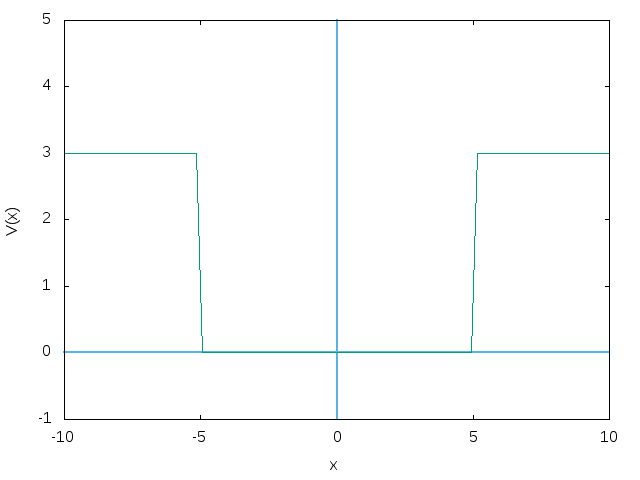
\includegraphics[width=0.7\textwidth]
  		{images/buca.png}
  		\caption{\label{fig:my-label2} esempio di buca simmetrica}}
  \end{figure}
 
 \textbf{Nota bene:} qui abbiamo posto gli estremi della buca simmetrici rispetto all'asse y e $V_0$ positivo, ma uno degli estremi potrebbe tranquillamente essere posto su $x=0$, cambierebbe solo il calcolo delle autofunzioni per questioni di simmetria, come vedremo più avanti. In casi diversi (ex. una buca con $V(x)\neq 0 \; \forall x \in[c,d]$ entrambi maggiori di 0) è sempre possibile applicare cambi di variabile per ricondursi ai primi due casi, decisamente più comodi da studiare.
  
 Che forma avranno le autofunzioni? Prima di risolvere l'equazione di Schrödinger, studiamo la continuità. Sappiamo che:
 
 \begin{align}
 \psi''(x)= \frac{2m}{\hbar^2}[V(x)-E]\psi(x) \\
 \downarrow \nonumber \\
 \psi'(\epsilon) - \psi'(0)= \frac{2m}{\hbar^2} \int_{0}^{\epsilon}dx [V(x)-E]\psi(x)
  \end{align}
 
 
 Siccome $V(x), \, \psi(x)$ sono limitate in $(0,\epsilon)$ avremo che il secondo termine $\rightarrow 0$ per $\epsilon \rightarrow 0$ da cui segue che
 
 \begin{align}
 \lim_{\epsilon \rightarrow 0}\psi'(\epsilon)= \psi'(0)
 \end{align}
 
 Quindi $\psi'(x)$ è continua ai bordi, e per conseguenza lo è anche $\psi(x)$.
\newpage 
 Studiamo ora l'eq. di Schrödinger nel caso di buca simmetrica:
 
 \begin{align}
 \psi''(x)=
 \left\{
\begin{array}{cc}
\frac{2mE}{\hbar}{}&\psi(x)\quad x\in [-a,a] \\
\frac{2m(V_0 - E)}{\hbar}&\psi(x) \quad x\notin [-a,a]
\end{array} 
 \right.
 \end{align}
 
per pulizia definiamo

\begin{align}
{}&k= \frac{\sqrt{2mE}}{\hbar} \\
&K= \frac{\sqrt{2m(V_0 - E)}}{\hbar}
\end{align}

Iniziamo studiando le \textbf{soluzioni pari}:

\begin{align}
 \psi_p(x)=
 \left\{
 \begin{array}{ccc}
 A\cos{kx}+ A'\sin{kx} \quad {}&x\in [-a,a] \\
 Be^{-Kx}+B'e^{+Kx} \quad &x>+a \\
 Ce^{+Kx}+C'e^{-Kx} \quad &x<-a
 \end{array} 
 \right.
\end{align}
 
Ricordando che $\psi(x)\in L_2$ abbiamo che
\begin{align}
B'= C'=0
\end{align}
e dal fatto che stiamo studiando le soluzioni pari ne segue che

\begin{align}
A'=0
\end{align}

E quindi in conclusione

\begin{align}
\psi_p(x)=
\left\{
\begin{array}{ccc}
A\cos{kx} \quad {}&x\in [-a,a] \\
Be^{-Kx} \quad &x>+a \\
Be^{-Kx} \quad &x<-a
\end{array} 
\right.
\end{align}

Siccome $\psi(x)$ è continua avremo anche che, per $x=a$ (discorso analogo per l'altro estremo):

\begin{align}
{}&\psi(a)\rightarrow A\cos{ka}= Be^{-Ka} \\
&\psi'(a)\rightarrow Ak\sin{ka}= KBe^{-Ka}
\end{align}

le cui soluzioni vengono da

\begin{align}
{}&A=B=0 \; \text{(soluzione banale)}\\
&k\tan{ka}=K
\end{align}


\newpage
Per le soluzioni dispari avremo invece

\begin{align}
\psi_d(x)=
\left\{
\begin{array}{ccc}
A\sin{kx} \quad {}&x\in [-a,a] \\
+Be^{-Kx} \quad &x>+a \\
-Be^{+Kx} \quad &x<-a
\end{array} 
\right.
\end{align}

con soluzioni

\begin{align}
{}&A=B=0 \; \text{(soluzione banale)}\\
&\frac{k}{\tan{ka}}=-K
\end{align}
 
di nuovo, per pulizia di notazione, definiamo

\begin{align}
\xi=ka \\
\eta= Ka
\end{align}

e possiamo ora scrivere che

\begin{align}
{}&\eta_p= \xi \tan{\xi} \quad \; \text{soluzioni pari} \\
&\eta_d= -\frac{\xi}{\tan{\xi}}  \quad \text{soluzioni dispari}
\end{align}

e possiamo infine ricavare le soluzioni degli stati legati, che ricaviamo dalle intersezioni di $\eta_p$ e $\eta_d$ con

\begin{align}
\xi^2 + \eta^2 = \frac{2mV_0a^2}{\hbar^2}
\end{align}

*INSERIRE GRAFICO*

si nota come il numero di stati legati sia finito. Ad esempio se

\begin{align}
\frac{2mV_0a^2}{\hbar^2} <\frac{\pi^2}{4}
\end{align}

avremo solo uno stato pari, e per averne almeno uno dispari bisogna andare oltre $\frac{\pi^2}{4}$.

\newpage

\subsection{Caso di buca infinita}

Si parla di buca infinita quando il potenziale ha forma

\begin{align}
V(x)= \left\{
\begin{array}{cc}
0 \quad {}&x \in [-a,a]\\
+\infty  &x \notin [-a,a]
\end{array}
\right.
\end{align}

In questo caso, guardando il grafico precedente, notiamo che

\begin{align}
ka \rightarrow \frac{\pi}{2}
\end{align}

da cui le soluzioni prendono la forma

\begin{align}
\psi(x)=
\left\{
\begin{array}{ccc}
A\cos{kx} \quad {}& x\in [-a,a] \\
+Be^{-K(x-a)} \quad &x>+a \\
-Be^{+K(x+a)} \quad &x<-a
\end{array} 
\right.
\end{align}

Ma $\cos{\frac{\pi}{2}}=0$, e quindi

\begin{align}
\psi(x)=
\left\{
\begin{array}{ccc}
A\cos{\frac{\pi x}{2a}} \quad {}& x\in [-a,a] \\
0 &x\notin [-a,a]
\end{array} 
\right.
\end{align}

Studiamo le soluzioni dentro la buca. Prendiamo una buca $[0,a]$ e imponiamo

\begin{align}
\left\{
\begin{array}{ccc}
\psi_n(a)= \psi_n(-a)=0\\
V_0=+\infty \qquad \qquad \;\,\\
|x|>a \quad \qquad \qquad \;\;
\end{array} 
\right.
\end{align}

Questo significa che presa

\begin{align}
\psi''(x)= \frac{2mE}{\hbar^2}\psi(x) \rightarrow \psi(x)= A\sin{kx}+B\cos{kx}
\end{align}

considerando le condizioni ai bordi, e al fatto che è buca antisimmetrica bisogna porre

\begin{align}
\psi(a)=\psi(0)=0 \quad ; \quad B=0
\end{align}

da cui

\begin{align}
A\sin{ka}=0 \rightarrow ka=n\pi \rightarrow k = \frac{n\pi}{a} \quad ; \quad n>0
\end{align}

e quindi per buche antisimmetriche si ottiene

\begin{align}
{}&\psi_n(x)= A\sin{\frac{n\pi x}{a}} \\
&ka=n\pi \rightarrow \frac{\sqrt{2mE_n}}{\hbar}a= n\pi \rightarrow \frac{2mE_n}{\hbar^2}a^2= n^2\pi^2 \nonumber \\
&\downarrow \nonumber\\
&E_n= \frac{\hbar^2 \pi^2}{2ma^2}n^2
\end{align}

Mentre per le simmetriche (del tipo $ [-a,a]$) basta sostituire il seno col coseno.

\newpage

\section{Barriera di potenziale ed effetto tunnel}

Si parla di barriera di potenziale quando si ha un sistema del tipo

\begin{align}
V(x)= \left\{
\begin{array}{ccc}
0 \quad {}&x\notin[0,L]\\
V_0\quad &x\in[0,L]
\end{array} 
\right.
\end{align}

\begin{figure}[!htb]
	\center{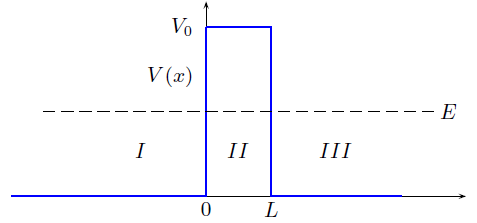
\includegraphics[width=0.6\textwidth]
		{images/BP.png}
		}
\end{figure}

Classicamente parlando, tutte le particelle con $E<V_0$ provenienti da ambo i lati verrebbero semplicemente riflesse indietro. Quantisticamente ciò non è detto, e si parla di \textbf{effetto tunnel}.

Questo perché le regioni ai lati della barriera sono di tipo I, e hanno quindi autovalori continui e discreti, da cui

\begin{align}
\psi(x)=\left\{
\begin{array}{cc}
Ae^{ikx} + A'e^{-ikx} 	\quad x\leq 0\\
Ce^{ikx} + C'e^{-ikx} 	\quad x\geq a
\end{array}
\right.
\end{align}

Siccome l'eq. di Schrödinger è di 2o grado, solo due dei coefficienti di $\psi(x)$ saranno linearmente indipendenti, a seconda della direzione della particella.

Studiamo il problema con una particella che arriva da sinistra. In questo caso, affinché la soluzione sia limitata deve essere

\begin{align}
A\neq 0 \quad;\quad C'=0
\end{align}

\begin{align}
\psi(x)=\left\{
\begin{array}{cc}
e^{ikx} + A'e^{-ikx} 	\quad {}&x\leq 0\\
Ce^{ikx}  \qquad \quad \; \; 	\quad &x\geq a
\end{array}
\right.
\end{align}


Deve essere $C\neq 0$ perché le soluzioni non poso annullarsi con la derivata in un punto, figuriamoci in un intervallo, mentre $A=1$ è dovuto all'omogeneità dell'equazione.

Come possiamo vedere \textbf{è possibile che la particella si trovi a destra della barriera, pur venendo da sinistra}.

Nell'ottica della barriera di potenziale possiamo dare i seguenti nomi ai coefficienti

\begin{align}
|A|^2=1 \qquad {}&\text{Coefficiente di incisione} \\
|A'|^2 \qquad \quad \;\; &\text{Coefficiente di riflessione} \\
|C|^2  \qquad \quad \;\;\, &\text{Coefficiente di trasmissione}
\end{align}

A' e C dipendono dal potenziale, ma vale sempre la relazione 

\begin{align}
|A'|^2+|C|^2=1
\end{align}

Per dimostrarlo partiamo dal caso 3D:

\begin{align}
-\frac{\hbar^2}{2m}\Delta \psi + V \psi= E \psi \quad;\quad \Delta = \nabla^2= \left(
\frac{\partial^2}{\partial x^2} + \frac{\partial^2}{\partial y^2} + \frac{\partial^2}{\partial z^2}
\right)
\end{align}

Considerata la coniugata:


\begin{align}
-\frac{\hbar^2}{2m}\Delta \psi^* + V \psi^*= E \psi^*
\end{align}

Moltiplichiamo prima l'una per l'altra e viceversa e sottraiamo i due risultati, ottenendo:

\begin{align}
\psi^*\Delta \psi - \psi \Delta \psi^*=0 \rightarrow \text{div}(\psi^*\Delta \psi - \psi \Delta \psi^*)=0
\end{align}

Definiamo la \textbf{corrente di probabilità} come:

\begin{align}
j = -\frac{i\hbar}{2m}(\psi^*\Delta \psi - \psi \Delta \psi^*)
\end{align}

da cui, se $\psi=\psi^*$ otteniamo l'\textbf{equazione di continuità}:

\begin{align}
\text{div} j = 0
\end{align}

Che ci porta ad avere, nel caso 1D:

\begin{align}
\frac{\partial}{\partial x}(\psi^*\Delta \psi - \psi \Delta \psi^*)= 0
\end{align}


Integrando su di un intervallo $[x_1,x_2]$ si ottiene

\begin{align}
\text{Im}(\psi^*(x_1)\psi'(x_1))=\text{Im}(\psi(x_2)\psi'x^*(x_2))
\end{align}

Qualora $x_1 <0 \, ,\, x_2>a$ risulta

\begin{align}
{}&\text{Im}[(e^{-ikx_1} + Ae^{-ikx_1})   (ike^{ikx_1} -ikA e^{-ikx_1})] = \text{Im}[Ce^{ikx_2}(-i)kCe^{-ikx_2}] \nonumber \\
&\downarrow \nonumber \\
&\text{Im}[ik - ikA e^{-2ikx_1} + ikA e^{-2ikx_1} -ik |A|^2 ] = \text{Im}[C(-i)kC] \nonumber \\
&\downarrow \nonumber \\
& \text{Im}[ik -ik |A|^2 ] = \text{Im}[-ik|C|^2]\nonumber \\
&\downarrow \nonumber \\
& \text{Im}[ik(1 -|A|^2) ] = \text{Im}[-ik|C|^2]\nonumber \\
&\downarrow \nonumber \\
& 1- |A|^2=|C|^2 \rightarrow |A|^2+|C|^2=1
\end{align}


Svolgendo conti che in queste dispense NON faremo perché mi rifiuto CATEGORICAMENTE è possibile ricavare il valore di $|C|^2$, che riportiamo di seguito:

\begin{align}
|C|^2 = \frac{4E(V_0 - E)}{4E(V_0 - E) - V_0^2 \sinh{Ka}} \quad;\quad K= \frac{\sqrt{2m(V_0 - E)}}{\hbar}
\end{align}


